\section{Fonctionnalités - Calcul séquentiel}

Dans cete partie nous verrons la structure du programme de base ainsi que ses performances en mode séquentiel

\subsection{Fonctionnalités du programme}
Tout d'abord, quelques rappels sur la structure du programme et des algorithmes de calcul sur les particules.

\paragraph{Mouvement des particules}
La position et la vitesse de chaque atome sont stockées dans deux tableaux de float distincts. Dans ces tableaux, sont d'abord stockées à la suite les composantes suivant x de tous les atomes, ensuite les composantes suivant y, puis selon z en fin de tableau.

A chaque itération de calcul, la fonction $seq\_move()$ met à jour le tableau des positions en ajoutant simplement à la position de chaque atome, sa vitesse.
Le calcul s'effectue ainsi en temps linéaire.

\paragraph{Rebond sur les murs}
Deux valeurs $min\_ext$ et $max\_ext$ délimitent un espace contenant les atomes. Pour garantir le fait que les atomes restent dans cet espace, la fonction $seq\_bounce()$ fait rebondir les atomes lorsqu'ils atteignent les limites de l'espace.
Pour réaliser le rebond, en testant pour chaque atome si l'un des bords de l'espace a été dépassé, et dans ce cas, on se contente de remplacer la composante de la vitesse selon le côté dépassé, par son opposé. Ce qui s'effectue également en temps linéaire.

\paragraph{Potentiel de Lennard-Jones}
L'interaction entre les atomes est calculée grâce au potentiel de Lennard-Jones. Celui-ci dépend de la distance qui sépare un couple d'atomes considéré.
Pour éviter des calculs insignifiants, on se donne une distance maximale (ou rayon de coupure). Si la distance entre deux atomes dépasse ce rayon, le calcul de la force est négligée.

L'algorithme de base est de complexité en temps quadratique.

\subsection{Performances}
Nous allons vous présenter dans cette partie les performances obtenues lors d'une exécution séquentielle du programme. 
La configuration matérielle utilisée lors des tests est la suivante :
\begin{itemize}
\item{CPU :} Intel Core i5 2500K - 4 c\oe urs
\item{GPU :} Nvidia GeForce 560Ti - 384 c\oe urs
\end{itemize} 
\vspace {0.4cm}
\par
Le graphique qui suivant montre le temps d'exécution d'une itération en fonction du nombre d'atomes simulés (Moyenne sur 100 itérations)

\begin{figure}[!h]
    \centering
    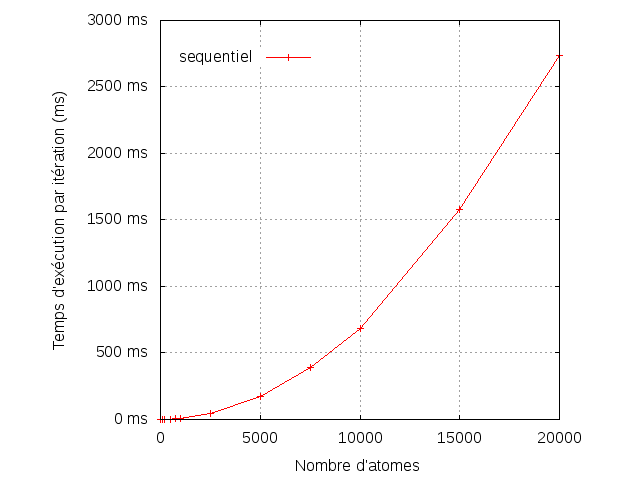
\includegraphics[scale=0.7]{./img/seq.png}
    \caption{Temps d'exécution d'une itération en fonction du nombre d'atomes}
\end{figure}

On peut remarquer que le programme actuel est très rapidement à la peine lorsque le nombre d'atomes augmente. A tel point qu'il n'est pas possible par exemple d'effectuer de simulation sur le fichier de configuration $biochoc1$ (contenant plus de 40000 atomes) en un temps raisonnable. 
La forme de la courbe laisse fortement entrevoir une complexité quadratique (liée au calcul de la force).


Dans le même temps, nous ne comptons sur les quelques optimisations que le compilateur ou que le matériel peuvent trouver. A ceux-ci près, le programme est entièrement séquentiel, et nous sommes très en deçà des capacités théoriques du matériel.
De plus, la quasi totalité du temps d'exécution est dû au calcul de la force, ce qui n'est pas surprenant puisqu'il s'effectue en $O(n^2)$ alors que les autres processus ne sont qu'en $O(n)$.
Nous voyons ainsi que pour obtenir de meilleurs résultats, il est nécéssaire de revoir l'algorithme de calcul de la force. C'est l'objet des parties qui vont suivre.

\begin{figure}[!h]
    \centering
    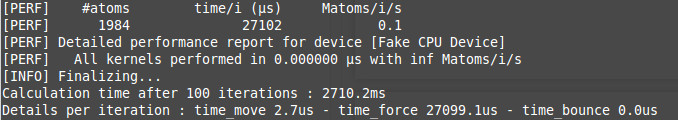
\includegraphics[scale=0.4]{./img/seqtime.jpg}
    \caption{Détails du temps de calcul sur 100 itérations de choc1.conf}
\end{figure}